\documentclass{article}
%\documentclass{IEEETran}

%\usepackage{anysize}
%\usepackage[left=1.9cm,right=1.9cm,top=2.54cm,bottom=1.9cm]{geometry}
%\usepackage{sectsty}
%\sectionfont{\normalsize \bf}
%\subsectionfont{\normalsize \bf}

%\IEEEoverridecommandlockouts  
%\overrideIEEEmargins

%\usepackage{siunitx}
\usepackage{setspace} 
%\doublespacing
\usepackage{cite}
\usepackage{amsmath}
\usepackage{amsthm}
\theoremstyle{remark}
\newtheorem{assumption}{Assumption}
\theoremstyle{remark}
\newtheorem{remark}{Remark}
\theoremstyle{remark}
\newtheorem{theorem}{Theorem}
\theoremstyle{remark}
\newtheorem{lemma}{Lemma}
\theoremstyle{remark}
\newtheorem{property}{Property}
\theoremstyle{remark}
\newtheorem{definition}{Definition}
\usepackage{graphicx}
\usepackage{fancyhdr}
\usepackage[bottom]{footmisc}
\usepackage{hyperref}
\usepackage{amssymb}
\usepackage{enumerate}
\usepackage{mathtools}

\usepackage{ifthen}
\DeclarePairedDelimiter{\norm}{\lVert}{\rVert}
\DeclarePairedDelimiter{\abs}{\lvert}{\rvert}%
% \DeclareMathOperator*{\argmax}{arg\,max} % thin space, limits underneath in displays
% \DeclareMathOperator*{\argmax}{argmax} % no space, limits underneath in displays
% \DeclareMathOperator{\argmax}{arg\,max} % thin space, limits on side in displays
\DeclareMathOperator{\argmax}{argmax} % no space, limits on side in displays
%===================================

\title{Invasive Species Management using Fast Feature Selection for Linear Value Function Approximation}

\makeatletter
\let\@fnsymbol\@arabic
\makeatother
\author{Soheil}
\date{}
\begin{document}
\maketitle

\section*{Abstract}
Glossy Buckthorns are not native to the United States, and were introduced to here from the Europe. Not having a natural predator, these plants have spread wildly into the nature, especially in New England area. In this paper, we study the land management strategies regarding to dealing with spreading these species using Markov Decision Processes (MDPs). Here, we tried to find out the optimal policy using various Reinforcement Learning methods, in which we approximate the state-action value function using Least-Squares Temporal Difference Q-function.

\section*{Invasive Species Management}

After introducing to a new environment, invasive plants start to grow up and produce seeds. The seeds fall off on the ground and create the plant's seed bank. Depending on the weather condition, some of these seeds germinate, some stay inactive in the seed bank, and some get transfered in the vicinity by wind, animals, and through other means. From the germinated seeds, some make juvenile, and later adult plants, and some die for various reasons. Adults make fruits, and produce seeds, and this cycle goes on forever.

Not having a natural predator drastically increases the chance of survival and the rates in which the plants make it to the next step in the cycle. If this cycle continues, all the resources of a region will be used by the invasive plant. In invasive species management, we are looking for effective ways to tackle the problem by removing the invasive plants in a right time. However, solving the issue sometimes means controlling the population of the invasive plant, sometimes means completely removing the invasive species from the region, and sometimes means leaving them to grow. 

\section*{Modeling the Costs}

In finding optimal policy, prior knowledge about the costs of taking different actions in each state is very crucial. It is usually the case that there are a few available methods for removing the invasive plant, each of which has a different cost and effectiveness, depending on the timing and the state that the system is at. So, at each point in time, we have to make a decision to pick an action from the list of all available actions, in which the total cost of our actions will be determined after an episode of experiment is finished. These problems are best represented by MDPs.

Although there are various types of treatment for dealing with Glossy Buckthorns, only one treatment is considered in this study, cutting and spraying the bushes. So, when we are talking about treating a region, what we really mean is cutting and spraying all bushes in that cell. This action has only one cost associated with it, and that is the accumulative cost of cutting and spraying in that area (later on, we show this cost with $c_1$). In general, we only consider two actions in this paper: a) not taking action ($a_0$), and b) taking action and killing bushes with cutting and spraying ($a_1$).

Not taking action means leaving the bushes in the area and letting them to grow. This action might not have immediate cost, but after some years of taking no actions, the system might be out of control and we might face some catastrophic economical results. This is usually because the invasive plants are so established in the region that it is going to be extremely difficult to get rid of them. They consume most of the available resources, from taking necessary mineral nutrition to grow off the ground, to blocking sun and preventing other plants from growing. This is horrible for lands that are primarily used by humans to grow trees, and we are trying to prevent these situations in invasive species management.

Economic modeling of invasive species management is very complicated. It is hard to represent the costs in terms of invasive plant's population, and is not the subject of this paper. The model that is used here is simply a threshold. When the population of Glossy Buckthorns grow bigger than a threshold, we have the cost of presence for each plant. But, in populations below the threshold, the cost of presence is zero. The total cost at each time for a region, is the summation of the cost of action, and the cost the presence, which is obtained by the current population of Glossy Buckthorns.

We can formulate this as following. $R_a$ is the cost of taking action $a$, as represented by
\[
  R_a = \left\{ 
  \begin{array}{lr}
    0 & a_0  \\
    c_1 & a_1
  \end{array}
  \right.
\]
and, $R_s$ is the cost of being at state $s$ (or having population $s_{pop}$)
\[
  R_s = \left\{
  \begin{array}{lr}
    0 & s_{pop} < Threshold \\
    s_{pop} c_2 & s_{pop} > Threshold
  \end{array}
  \right..
\]
where, $c_1$ and $c_2$ are constants. $c_1$ is the cost we considered for taking action $a_1$, and $c_2$ is the coefficient of the cost we need to pay for removing each plant, after reaching to a certain population. As stated before, the total cost is
\[
  R(s,a) = R_a + R_s.
\]

\section*{What is an optimal policy?}
After defining a cost function for our MDP, it is very important to understand how this cost function can impact the optimal policy in the system. It is usually impossible in RL to make sense of the problem in terms of policy, since we are dealing with an $N \times P$ hard issue. They are neither easy to solve nor understand by human.

Despite the difficulty of the problem, we are looking for some benchmark policies in order to evaluate the solutions we get from running different algorithms. One way to go around this problem is to consider some extreme cases. For instance, consider the case that the cost of presence is so high for the system in comparison to the cost of treatment, that we prefer to take action $a_1$ for all states. Taking action 1 is an optimal policy for this case, since it leads to less plants for next time steps, which means less cost of presence, and consequently, less total cost.

For the next extreme case, consider when the cost of treatment is so high in compared with the cost of presence that we prefer to let the plants grow. In this case, the optimal policy is to always take action $a_0$, which is doing nothing. These two extreme cases are used in this study as a benchmark, since we know the outcome we should be expecting from the optimal policy finder algorithm.


To better see the extreme cases, we design two experiments, and illustrate the problem using plots. In the first experiment, we increase the cost of presence of the plant from 5 to 50, with an interval of 5, and keep the cost of treatment on 10. Then we obtain the cost for each policy by calling the simulator with the policy (figure \ref{fig:presence}). We run the simulator for a large number of episodes (100 episodes of 200 steps), and take the average cost of simulations as the cost of respective policy. In the second experiment, the cost of treatment is increased from 5 to 50 with an interval of 5, and the cost of presence is kept constant at 10 (figure \ref{fig:treatment}), and we follow the same procedure to obtain the cost of the policy.


\begin{figure}
  \centering
  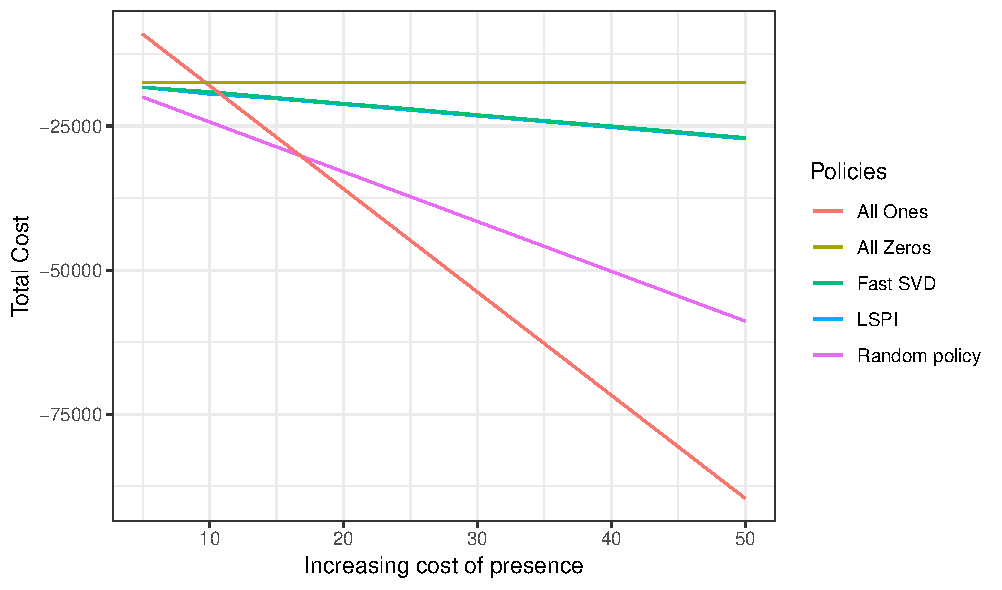
\includegraphics[scale=.8]{increasing_cost_treatment.pdf}
  \caption{Increasing the cost of treatment}
  \label{fig:treatment}
\end{figure}



\begin{figure}
  \centering
  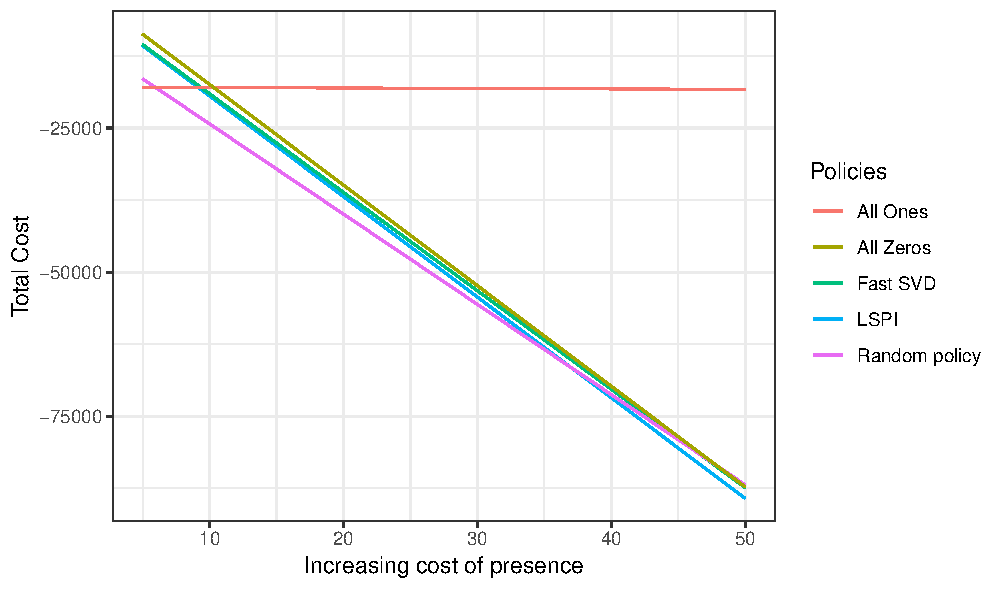
\includegraphics[scale=.8]{increasing_cost_presence.pdf}
  \caption{Increasing the cost of presence}
  \label{fig:presence}
\end{figure}





% \bibliographystyle{plain}
% \bibliography{invasive_species}
\end{document}


%===============================
%========== NOT TO RUN =========
\iffalse


\usepackage{titlesec}

\titleformat{\section}
  {\normalfont\Large\bfseries}   % The style of the section title
  {}                             % a prefix
  {0pt}                          % How much space exists between the prefix and the title
  {Section \thesection:\quad}    % How the section is represented

% Starred variant
\titleformat{name=\section,numberless}
  {\normalfont\Large\bfseries}
  {}
  {0pt}
  {}
  

asdasd \cite{1013341}. Fig.~\ref{Fig_Example}.

{\fontfamily{pcr}\selectfont 
run files}

\begin{enumerate}
  \item The labels consists of sequential numbers.
  \item The numbers starts at 1 with every call to the enumerate environment.
\end{enumerate}

\begin{itemize}

\end{itemize}

======== HYPERLINK =============
Find the \texttt{run files} for all variants in \href{https://github.com/SHi-ON/InfoRet/tree/master/results/Assignment_4}{here}


====== FIGURES ========

\begin{figure}
	\centering
	\includegraphics[scale=.40]{Fig_Example.pdf}
	\caption{Example.}
	\label{Fig_Example}
\end{figure}

\input{second}

========= EQUATIONS =============

\begin{equation}
\left\|\frac{\partial V}{\partial\mathbf{x}_1}\right\|\left\|\mathbf{x}_1\right\|\leq c_1V\quad \text{for}\; \left\|\mathbf{x}_1\right\|\geq c_2
\end{equation}


============ TABLES =============

\begin{tabular}{ |p{3cm}|p{3cm}|p{3cm}|  }
\hline
\multicolumn{3}{|c|}{Country List} \\
\hline
Country Name     or Area Name& ISO ALPHA 2 Code &ISO ALPHA 3 \\
\hline
Afghanistan & AF &AFG \\
Aland Islands & AX   & ALA \\
Albania &AL & ALB \\
Algeria    &DZ & DZA \\
American Samoa & AS & ASM \\
Andorra & AD & AND   \\
Angola & AO & AGO \\
\hline
\end{tabular}

\begin{center}
\begin{tabular}{ |c|c|c| } 
 \hline
 cell1 & cell2 & cell3 \\ 
 cell4 & cell5 & cell6 \\ 
 cell7 & cell8 & cell9 \\ 
 \hline
\end{tabular}
\end{center}




\begin{lstlisting}[language=Python, caption=Code's name]
import numpy as np
 
def incmatrix(genl1,genl2):
    m = len(genl1)
    n = len(genl2)
    M = None #to become the incidence matrix
    VT = np.zeros((n*m,1), int)  #dummy variable
\end{lstlisting}



\begin{verbatim}
Put your codes here!
\end{verbatim}
\fi
